\section{Research Object Digital Library}
\label{sec:rodl}

%This section presents the components that constitute the RODL, using a UML class diagram, and show how the user can utilize RODL using a UML sequence diagram.

The foundational service to preserve workflow-centric research objects is the Research Object Digital Library (RODL), which realizes the Storage and Lifecycle functionalities described in Section \ref{architecture}. It is a software system which collects, manages and preserves aggregations of scientific workflows and related objects and annotations, packed into research objects.

\begin{figure}[!hb]
\centering
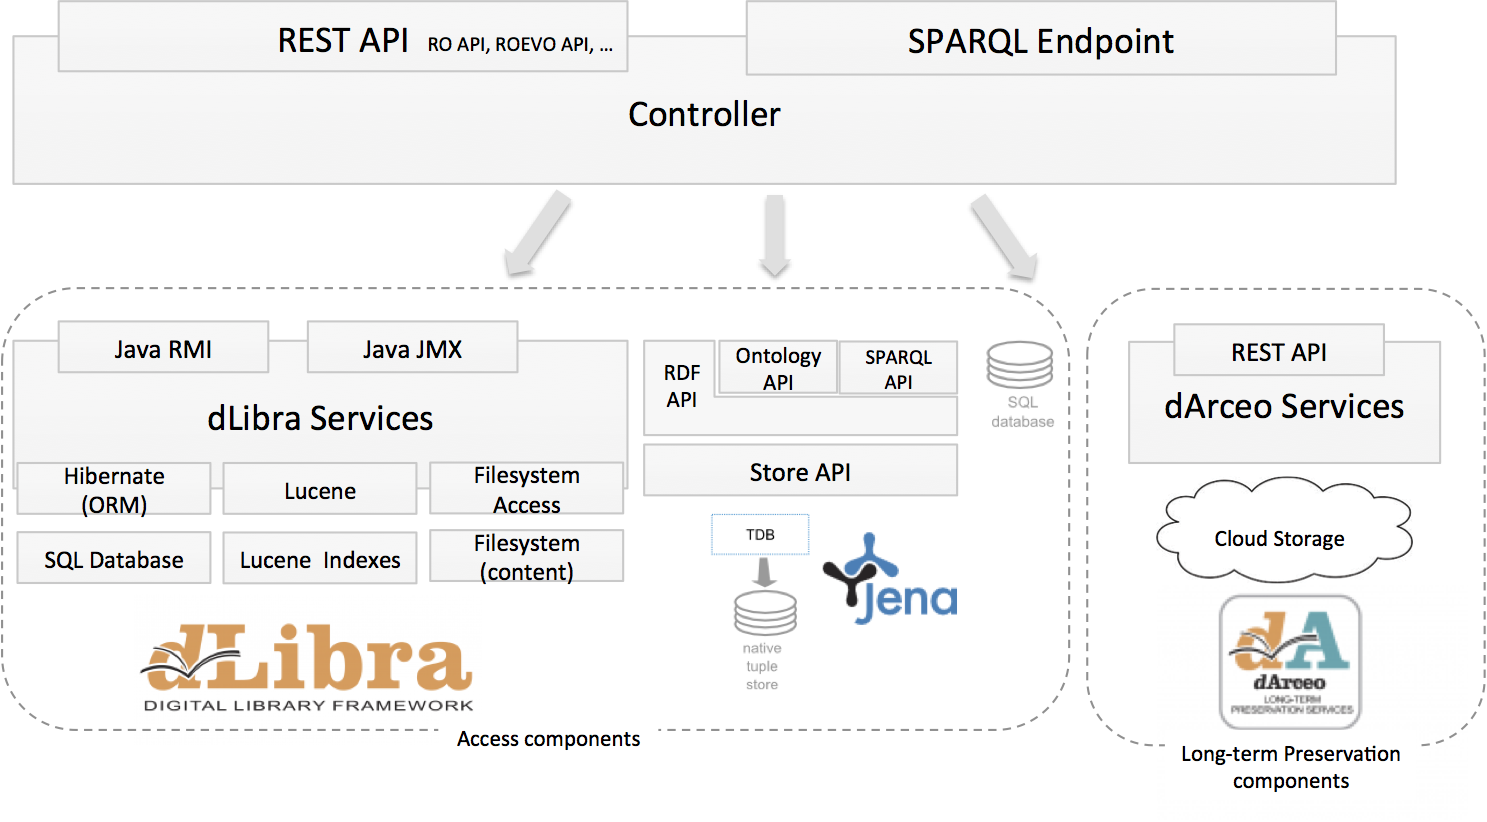
\includegraphics[width=\textwidth]{Figures\RODL-new.png}
\caption{Research Objects Digital Library internal component diagram}
\label{RODL}
\end{figure}


\subsection{The interfaces}

The main interface of RODL is a set of REST APIs, among which the two primary ones are the RO API \cite{RO-API} and the RO Evolution API \cite{RO-EVO-API}.

The RO API, also called the RO Storage and Retrieval API, defines the formats and links used to create and maintain research objects in the digital library. It is aligned with the RO model that is used to define research objects, and so it recognizes concepts such as aggregations, annotations and folders. The RO model ontology \cite{RO_model} is used to specify relations between different resources. Given that the semantic metadata are an important component of a research object, the RODL supports content negotiation for the metadata resources, including formats such as RDF/XML, Turtle and TriG.

The RO Evolution API defines the formats and links used to change the lifecycle stage of a research object, most importantly to create an immutable snapshot or archive from a mutable live research object, as well as to retrieve the evolution provenance of a research object. The API follows the RO evolution model \cite{w4fever_d321}, which is most visible in the evolution metadata that are generated for each state transition.

Additionally, RODL provides a SPARQL endpoint that allows performing SPARQL queries over HTTP to the metadata of all stored research objects. It also implements the Notification API \cite{Notification-API}, which defines links used to retrieve Atom feeds with notifications of events about any research object. For searching the contents of research objects a Solr REST API and the OpenSearch APIs are provided. Finally, RODL implements a custom User Management API \cite{UM-API} for registering users and generating OAuth 2 access tokens, providing the option of extending it with an access control layer in the future.



\subsection{The implementation}

One of the main design challenges related to the implementation of RODL was the need to support both live, dynamically changing research objects as well as immutable snapshots that are intended for a longterm preservation. With this in mind, the RODL has a modular structure that comprises the access components, the longterm components and the controller that manages the flow of data (see figure \ref{RODL}). For immutable research objects, they are stored in the longterm preservation repository once they are created. The live research objects, on the other hand, are pushed asynchronously after every change or periodically, depending on the configuration.

The access components are the storage backend - dLibra \cite{dLibra} - and the semantic metadata triplestore. dLibra provides file storage and retrieval functionalities, including file versioning and consistency checking. It has a built-in text search engine and it manages users and controls their access rights. It allows organizing stored objects into hierarchical structures and associating metadata at the level of object aggregations. It is also possible to use a built-in module for storing research objects directly in the filesystem.

The semantic metadata are additionally parsed and stored in the triplestore backed by Jena TDB \cite{Jena}. Jena TDB is an actively developed RDF store implementation, which provides good support for transactions, querying, cacheing and using named graphs. The use of a triplestore helps in RODL internal data processing and offers a standard query mechanism for RODL clients. It also provides a flexible mechanism for storing metadata about any component of a research object that is identiable via a URI, which apart from workflows and other resources, may include parts of workflows or external resources (e.g. web services, data sources).

The UML sequence diagrams illustrate the interactions between the controller, the storage backend and the triplestore for the basic operations of creating a research object and aggregating resources to it (\ref{ROCreate,RODelete,ResourceAdd,ResourceUpdate,ResourceDelete}). Creating immutable snapshots of research objects is a more complex process which involves copying the resources, recording their provenance, optional modifications by the user and finally releasing as a published, immutable object. Figure \ref{SnapshotClient} shows how RODL clients can perform these steps via the RO Evolution API. Figures \ref{SnapshotPerform,SnapshotFinalize} present the interaction between internal RODL components when performing the process of creating the snapshot.

The longterm preservation component is built on dArceo \cite{dArceo} - a system for longterm preservation of digital objects developed by PSNC. dArceo stores the objects and monitors their quality, alerting the administrators if necessary \ref{dArceoStore}. The standard monitoring activities include file format decay alerts and fixity checking but can be enhanced using a plugin mechanism. In case of RODL, dArceo periodically monitors the quality of research objects by calling the Checklist Evaluation and Stability Services \cite{Checklist-API,Stability-API} \ref{dArceoQuality}. If a change in quality is detected, notifications are generated as Atom feeds in compliance with the Notification API mentioned above. This helps detect and prevent workflow decay which occurs when an external resource or service used by the workflow becomes unavailable or is otherwise behaving differently.

dArceo gives the possibility to define migration plans that allow to perform a batch update of resources from one format to another, when necessary. In case of workflows, this may be applied for instance when a flat Taverna t2flow format should be converted to a complex scufl2 format (which, notabene, uses the RO model similarly to research objects). Other case could be a batch update of workflows that depend on a malfunctioning external resource.

Objects in dArceo can be stored on a range of backends, including specialized preservation repositories such as the Platon service \cite{Platon}, storing data in geographically distributed copies and guaranteeing their consistency.

A running instance of the RODL is available for testing at \url{http://sandbox.wf4ever-project.org/rodl/}. At the moment of writing, it holds more than 1300 research objects.


\begin{figure}[!hb]
\centering
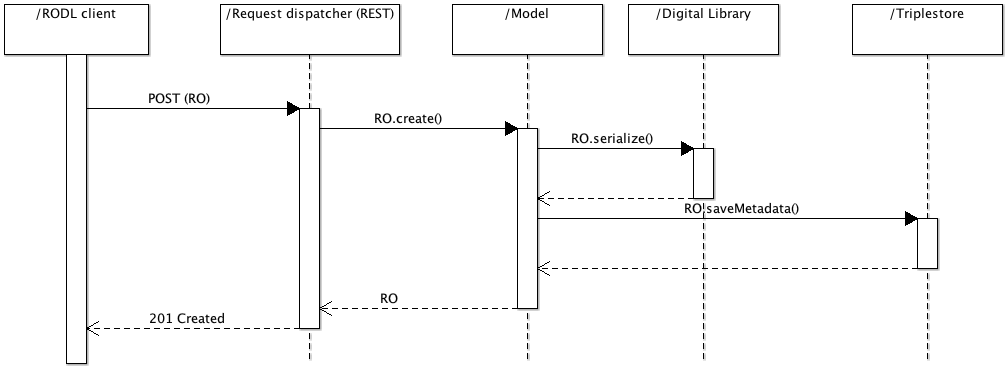
\includegraphics[width=\textwidth]{Figures\RODL\ROcreate.gif}
\caption{The sequence diagram for creating a research object in RODL}
\label{ROCreate}
\end{figure}

\begin{figure}[!hb]
\centering
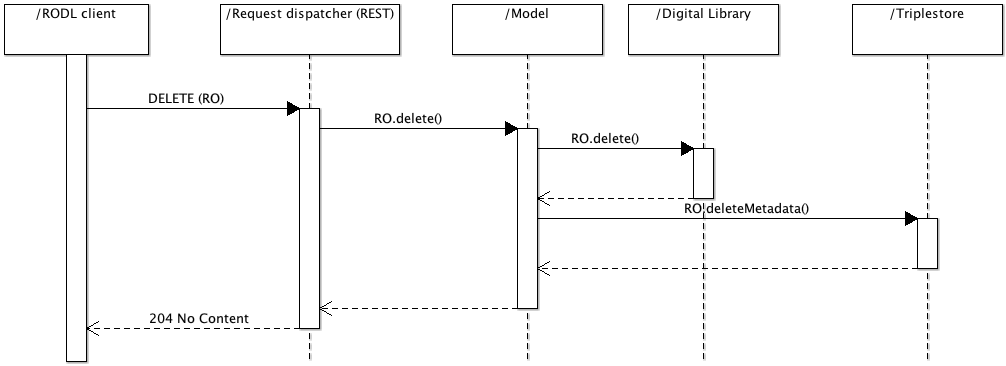
\includegraphics[width=\textwidth]{Figures\RODL\ROdelete.gif}
\caption{The sequence diagram for deleting a research object from RODL}
\label{RODelete}
\end{figure}

\begin{figure}[!hb]
\centering
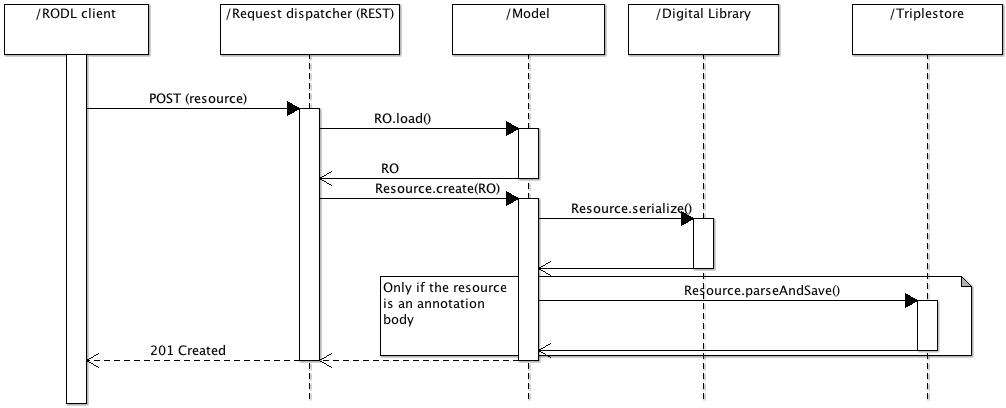
\includegraphics[width=\textwidth]{Figures\RODL\ResourceAdd.gif}
\caption{The sequence diagram for aggregating a new resource in a research object}
\label{ResourceAdd}
\end{figure}

\begin{figure}[!hb]
\centering
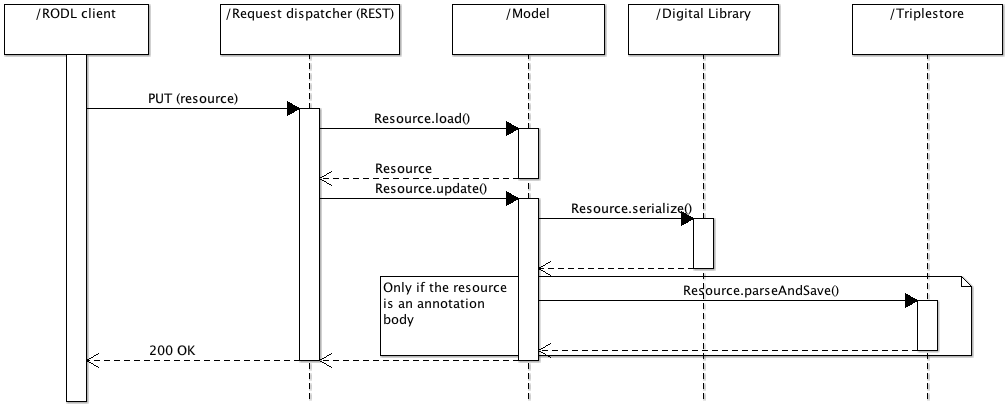
\includegraphics[width=\textwidth]{Figures\RODL\ResourceUpdate.gif}
\caption{The sequence diagram for updating an existing resource in a research object}
\label{ResourceUpdate}
\end{figure}

\begin{figure}[!hb]
\centering
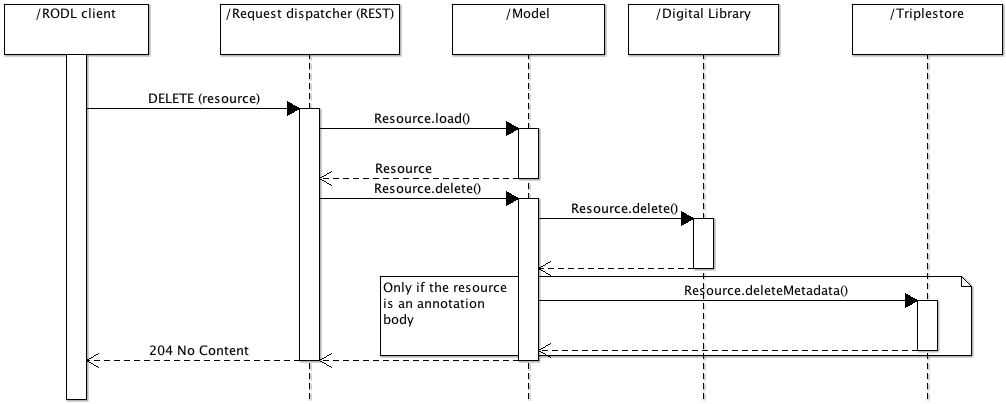
\includegraphics[width=\textwidth]{Figures\RODL\ResourceDelete.gif}
\caption{The sequence diagram for deleting a resource from a research object}
\label{ResourceDelete}
\end{figure}

\begin{figure}[!hb]
\centering
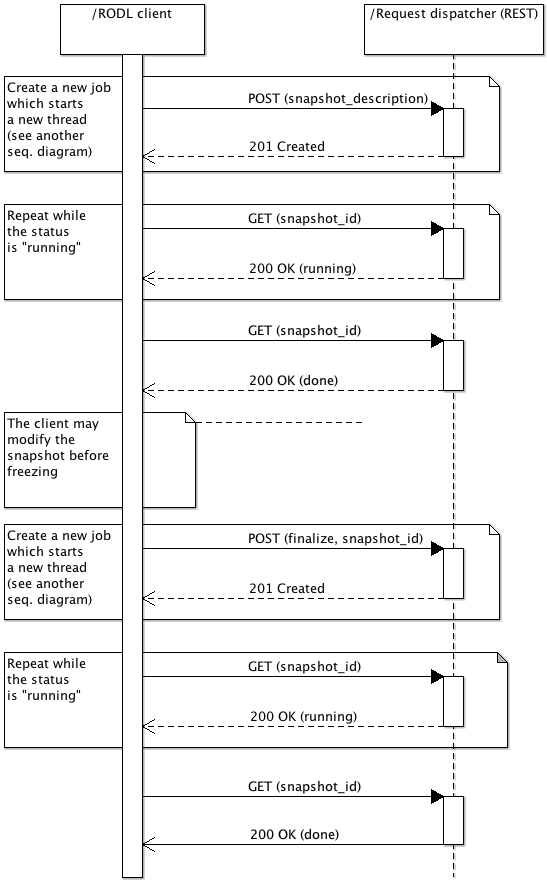
\includegraphics[width=\textwidth]{Figures\RODL\SnapshotClient.gif}
\caption{The sequence diagram for creating a snapshot or release from the RO Evolution API client perspective}
\label{SnapshotClient}
\end{figure}

\begin{figure}[!hb]
\centering
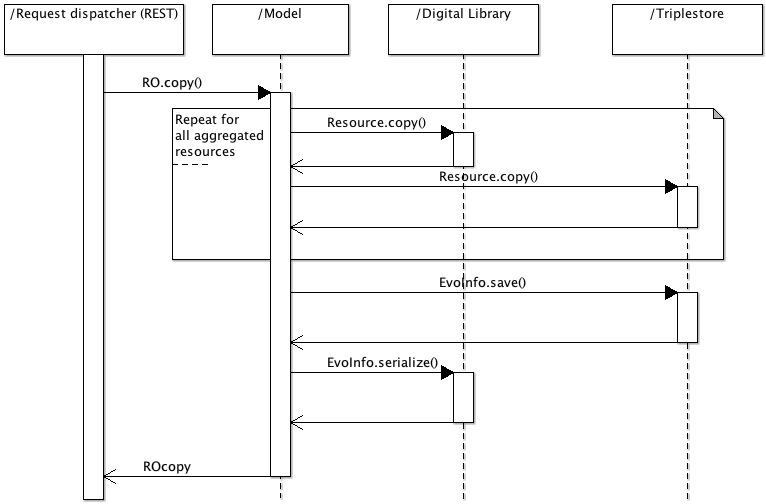
\includegraphics[width=\textwidth]{Figures\RODL\SnapshotPerform.gif}
\caption{The sequence diagram for preparing the snapshot of a research object}
\label{SnapshotPerform}
\end{figure}

\begin{figure}[!hb]
\centering
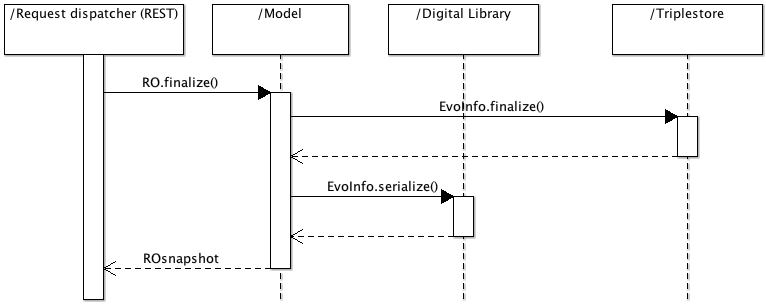
\includegraphics[width=\textwidth]{Figures\RODL\SnapshotFinalize.gif}
\caption{The sequence diagram for finalizing the snapshot and making it immutable}
\label{SnapshotFinalize}
\end{figure}

\begin{figure}[!hb]
\centering
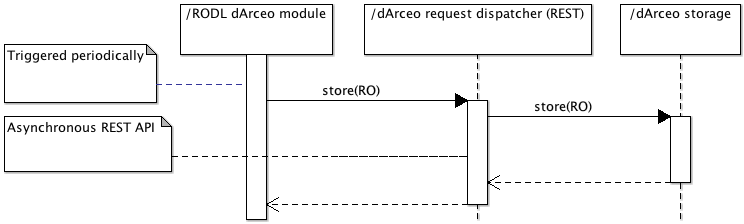
\includegraphics[width=\textwidth]{Figures\RODL\dArceoStore.gif}
\caption{The sequence diagram for storing research objects in dArceo}
\label{dArceoStore}
\end{figure}

\begin{figure}[!hb]
\centering
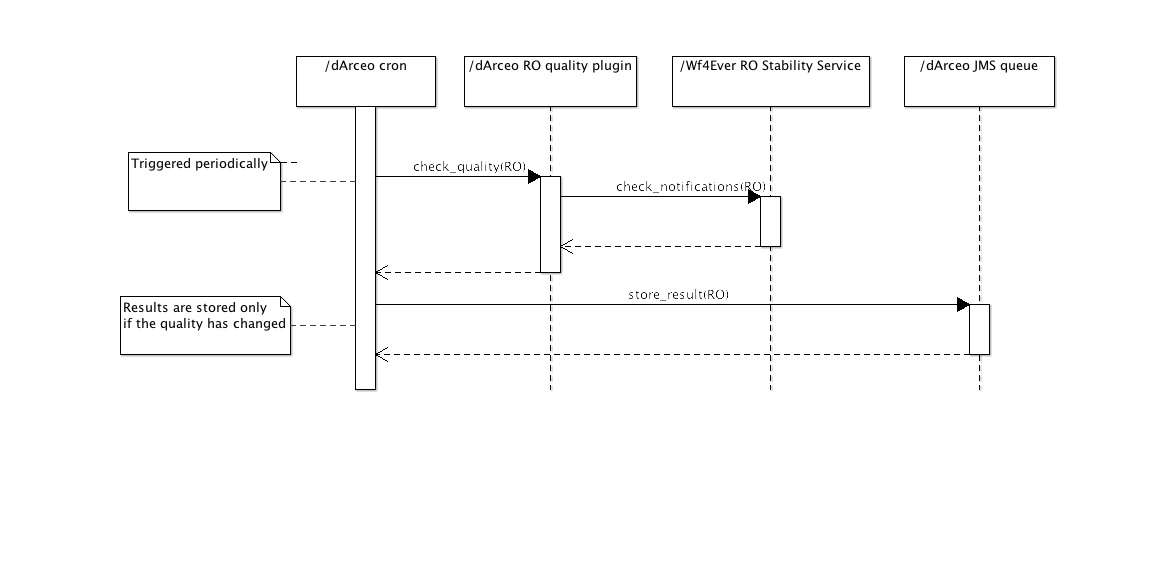
\includegraphics[width=\textwidth]{Figures\RODL\dArceoQuality.png}
\caption{The sequence diagram for checking the quality of research objects in dArceo}
\label{dArceoQuality}
\end{figure}

\subsection{RODL clients}

The use of a REST API as the primary interface of RODL shows the need for clients that can facilitate the interaction with RODL for the users. To this moment, the following clients support some or all of the RO APIs implemented by RODL.

The reference client of RODL is \textbf{the RO Portal}, developed alongside RODL to test new features and expose all available functionalities. It is a web application running at \url{http://sandbox.wf4ever-project.org/portal}. Its main features are research object exploration and visualization; it also allows to create user accounts in RODL and generate access tokens for other clients. The RO Portal uses all APIs of RODL. Figure \ref{Portal} shows the main view of a research object in the RO Portal. The development version of \textbf{myExperiment} \cite{myExperiment} (\url{http://alpha.myExperiment.org}) uses RODL as a backend for storing packs. It uses the RO API. Finally, the \textbf{RO Manager} \cite{RO-Manager} is a command line tool that is primarily used to manage a research object stored on a local disk. It allows to push a research object to RODL via the RO API, as well as convert it into a snapshot in RODL.

\begin{figure}[!hb]
\centering
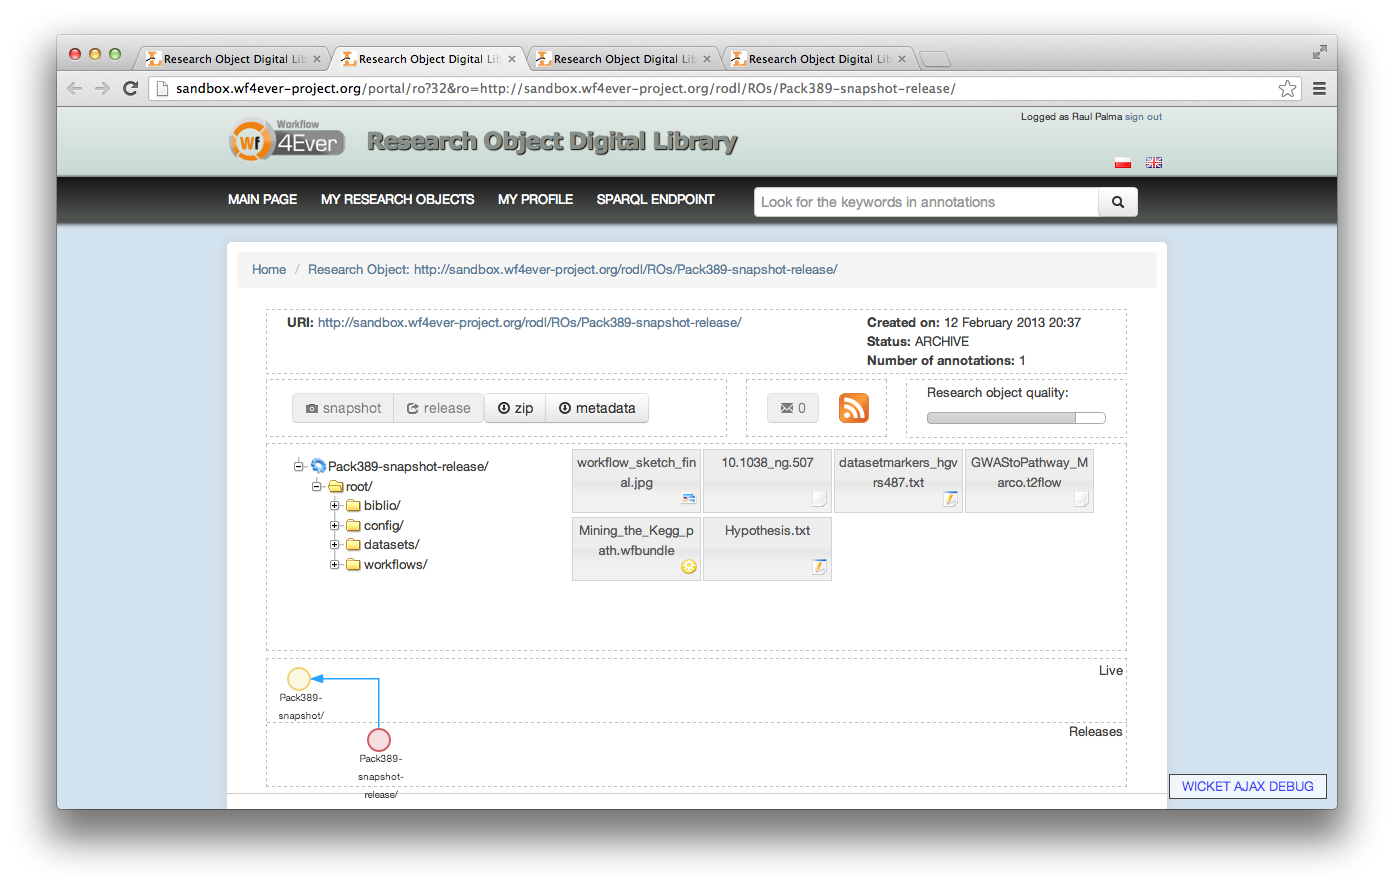
\includegraphics[width=0.98\textwidth]{Figures\RO-Portal-II.png}
\caption{The Research Object Portal}
\label{Portal}
\end{figure}
